\documentclass[11pt]{article}
\usepackage{common}
\usepackage{graphicx}
\title{Project Template}
\author{Anna Sophie Hilgard, Nick Hoernle, and Nikhila Ravi}
\begin{document}
\maketitle{}


\section{Introduction}

The goal of our project is to create a routing system for bicycle trips that takes into account more than just distance. Current map applications like Google often route cyclists through busy streets and intersections, resulting in unnecessarily dangerous trip and sometimes accidents. The algorithm we chose to use for this problem is A* search with a variety of cost functions and heuristics incorporating distance, safety of a given route, and changes in elevation (also important for biking but not information Google maps currently considers).

Additionally, we considered the problem of finding a central meeting place for two or more cyclists starting from different positions. To solve this optimization problem, we used k-beam search and simulated annealing.

The graph search problem is directly analogous to techniques and ideas from the class: using intersections as nodes in the graph and road segments connecting intersections as paths, we are able to construct the city maps as directed graphs. From there, we can use data generated from a variety of sources to come up with approximate costs associated with paths and related heuristics at nodes.

The optimization techniques we use are also direct applications of algorithms from the optimization portion of the course.

Problem-specific adaptations were largely limited to the collection and interpretation of relevant data and the development of a cost function and relevant heuristics.

\section{Background and Related Work}

While our problem was fairly straightforward, we did do some research to get ideas for potential cost attributes and data sources. Our initial formulation of the problem, for example, did not include elevation differencing, but reading previous studies led us to believe that this was an important criterion. \cite{pmbr}.

\section{Problem Specification}

The problem that we are solving is of the general class of graph search problems. Given a strongly connected graph, we seek to minimize some cost function $cost(\sum_{i=0}^n path_i)$ \\given that  $path_0 \in Connections_{starting node}$ \\$path_i, path_{i+1} \in Connections_{node_j}$ for some j, \\$path_i, path_{i-1} \in Connections_{node_k}$ for some k, and \\$path_n \in Connections_{target node}$

Specifically for our problem, we created three different cost functions:\\
Distance only: $cost(path_i)= length_i$ \\
Distance and safety only: $cost(path_i)  = \alpha* length_i * \beta * accidents_i$ \\
Distance, safety, and elevation: $cost(path_i) = \alpha* length_i * \beta * accidents_i + abs(\Delta elevation_i)$ \\

Where $\alpha$ and $\beta$ are multipliers to bring each of these values within what we find to be an appropriate range to generate reasonable results.

In the optimization portion of our project, we seek to minimize the total cost to all parties:\\
$min(\sum_j^n cost_j)$ where  $cost_j$ is the cost to participant j.

\section{Approach}

Data Structures: Our primary data structures are an intersection graph, which is stored as a Python dictionary, and a connection dictionary, which is also stored as a Python dictionary. The intersection graph maps nodes (intersections) by id to a list of paths (road segments) from that node. The connection dictionary maps a connection (road segment) to its source node, sink node, and various cost parameters (in our case distance, number of bicycle crashes on that road segment, and change in elevation over that road segment).

\begin{algorithm}[H]
  \begin{algorithmic}
    \Function{A-Star-Search}{$graph, start node, target node$}
    \State{$node \gets $a node with $ \textsc{state}=start node$}
    \State{$\textsc{path-cost} \gets \textbf{heuristic}(start node, target node)$}
    \State{$frontier\gets $ a priority queue ordered by $\textsc{path-cost} + \textbf{heuristic}(node, target node)$ with $node$ as the only element}
    \State{$explored \gets $ an empty set}
    \Loop 
    \If{$\textsc{Empty?}(frontier)$}
    \State \textbf{return failure}
    \EndIf
    \State{$node \gets \textsc{pop}(frontier)$ /*chooses the lowest cost+heuristic node in $frontier$ */}
     \If{$node == targetnode$}
    \State {\textbf{return} \textsc{solution}($node$)}
    \EndIf
    \State{add node.\textsc{State} to $explored$}
    \For{ \textbf{each} $path$ in \textsc{Paths}($node$)}
    \State{$child \gets$ \textbf{child-node}($node, path$)}
    \If {$child$.\textsc{State} is not in $explored$ or $frontier$}
    \State{$frontier \gets$ \textbf{insert}($child, frontier$)}
    \ElsIf  {$child$.\textsc{State} is in $frontier$ with higher \textsc{path-cost} + heuristic}
    \State{replace that $frontier$ node with $child$}
    \EndIf
    \EndFor
    \EndLoop
    \EndFunction{}
  \end{algorithmic}
  \caption{A-Star Search}
\end{algorithm}

\begin{algorithm}[H]
  \begin{algorithmic}
    \Function{Simulated Annealing Meeting Spot}{$graph, startingpts, cost, heuristic$}
    \If{$\textbf{length}(startingpts)<2$}
    \State \textbf{return error}
    \EndIf
    \State{$current \gets$ \textbf{mean}$(startingpts)$.\textsc{closest-node}}
    \State{$temperature \gets e^{10}$}
    \State{$\gamma \gets .5$ /*schedule to manage $temperature$ */}
    \While{$temperature > e^{-2}$}
      \State{$temperature \gets temperature*\gamma$}
      \State{$next \gets$ a randomly selected $child$ of $current$}
      \State{$current.\textsc{value} \gets \sum_{pt \in startingpts}\textbf{cost}(pt, centroid$)}
      \State{$next.\textsc{value} \gets \sum_{pt \in startingpts}\textbf{cost}(pt, next$)}
      \State{$\Delta E \gets next.\textsc{value} - current.\textsc{value}$}
      \If {$\Delta E > 0$}
      \State{$current \gets next$}
      \Else
       \State{$current \gets next$ with probability $e^{\Delta E / temperature}$}
      \EndIf   
    \EndWhile
    \EndFunction{}
  \end{algorithmic}
  \caption{Simulated Annealing Meeting Spot}
\end{algorithm}

\begin{algorithm}[H]
  \begin{algorithmic}
    \Function{K-Beam Search Meeting Spot}{$k, graph, startingpts, cost, heuristic$}
    \If{$\textbf{length}(startingpts)<2$}
    \State \textbf{return error}
    \EndIf \\
    \State{$\{candidatenodes\} \gets \,node\, \forall \,node \in graph $ s.t. \\ $node.x \ge min(startingpts.x) \& \,node.x \le max(startingpts.x) \&$ \\ $node.y \ge min(startingpts.y) \& \,node.y \le max(startingpts.y)$} \\
    
    \State{$point_i \gets$ a randomly selected $node \in \{candidatenodes\} \forall i \le k$}
    \State{$best.\textsc{value} \gets min_{i\le k}(\sum_{pt \in startingpts}\textbf{cost}(pt, point_i))$}
    \While{\textbf{True}}
      \State{$\{nextcosts \} \gets \sum_{pt \in startingpts}\textbf{cost}(pt, child_i) \forall i \le k, child_i \in \textsc{Paths}(point_i).endnode $}
      \State{$point_i \gets$ i-th least $node \in \{nextcosts\} \forall i \le k$}
      \State{$next.\textsc{value} \gets \sum_{pt \in startingpts}\textbf{cost}(pt, point_1$)}
      \If {$next.\textsc{value} < best.\textsc{value}$}
      \State{$best \gets next$}
      \Else
       \State{\textbf{break}}
      \EndIf   
      \State{\textbf{return} $best$}
    \EndWhile
    \EndFunction{}
  \end{algorithmic}
  \caption{K-Beam Search Meeting Spot}
\end{algorithm}



\section{Experiments}
Analysis, evaluation, and critique of the algorithm and your
implementation. Include a description of the testing data you used and
a discussion of examples that illustrate major features of your
system. Testing is a critical part of system construction, and the
scope of your testing will be an important component in our
evaluation. Discuss what you learned from the implementation.
\begin{itemize}

\item{Analysis:} To test our algorithms, we built graphs on GIS data from both Cambridge, MA and San Francisco, CA (supplemented with elevation and crash data collected from other sources as necessary). We ran both the single-path and meeting point algorithms for a variety of cost functions and start and end points and were pleased to see that the paths generated by our algorithms when taking into account safety and elevation factors do indeed seem to avoid busy intersections and steep hills in a reasonable way.

\begin{figure}[H]
\caption{Paths between nodes in San Francisco. Blue path optimizes for distance only, green path avoids previous bicycle accidents, and red path minimizes altitude changes. Overlaid with an altitude plot of San Francisco, we can clearly see the red path avoiding a hill.}
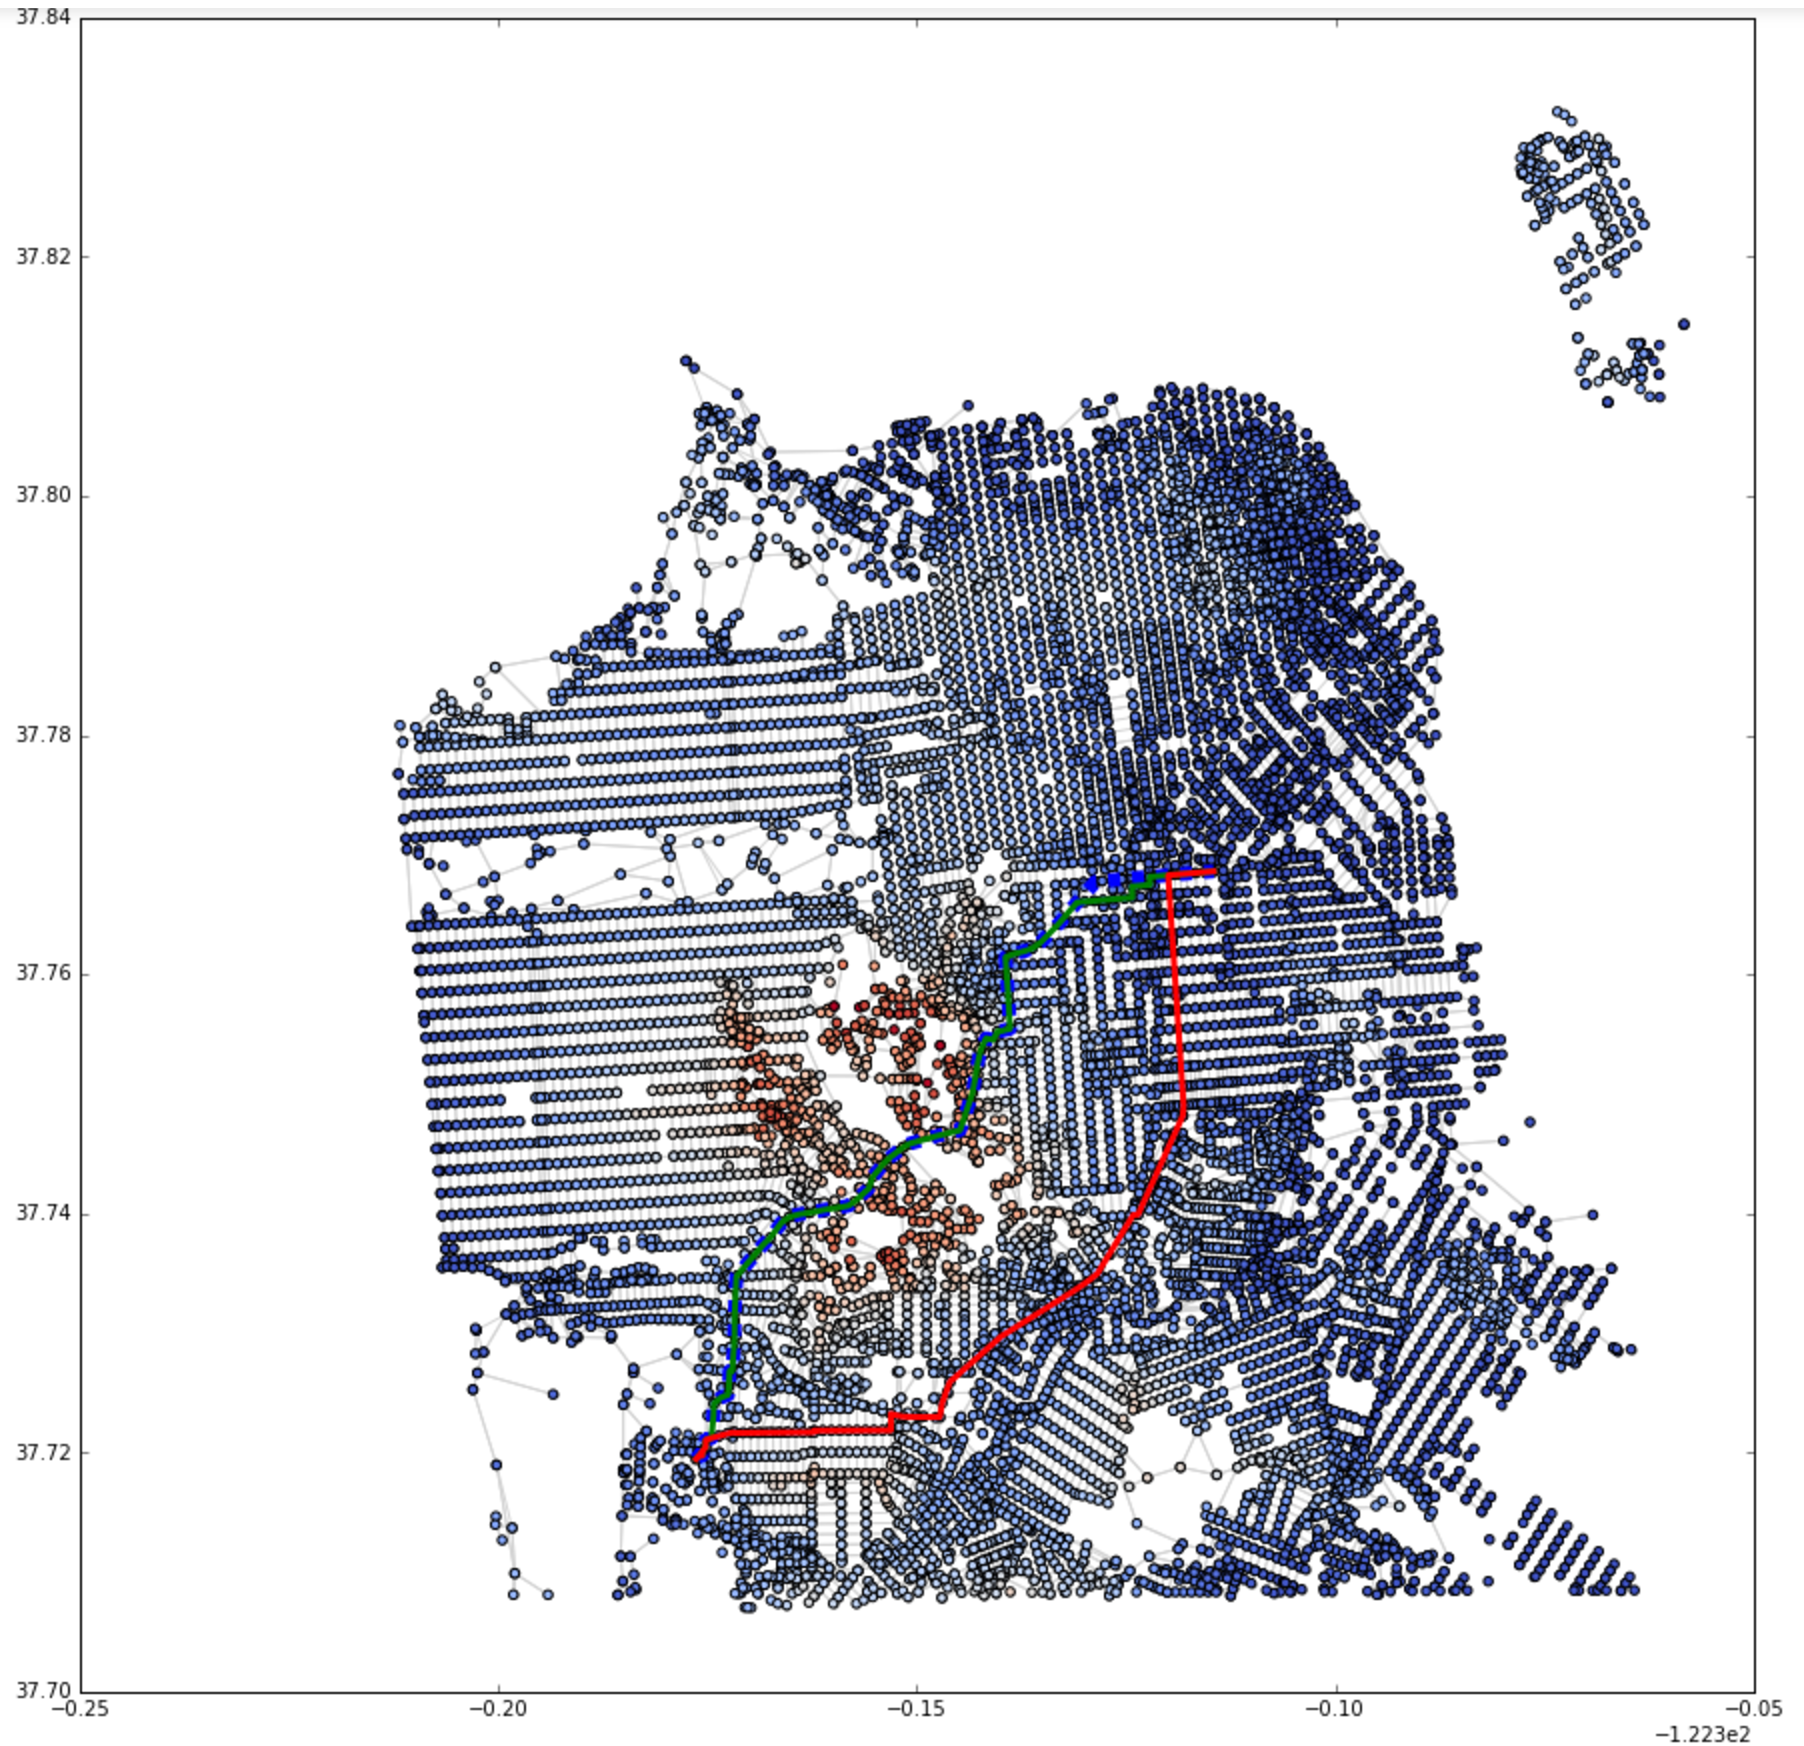
\includegraphics[width=0.6\textwidth]{sf_new_plot_2.png}
\end{figure}

\item{Evaluation:} We went through a few iterations of tuning the parameters in our cost function to get the appearance of the graphs to mimic what we think we'd want as cyclists. Because the cost in our problem is qualitative rather than explicitly quantitative, we were largely forced to estimate parameters based on what we thought would be reasonable rather than deriving them from empirical data of some sort. That said, we all felt that with our final parameters the algorithm was doing a reasonable job at generating routes we would want.

\item{Critique:} Our algorithms could have been made to run somewhat faster by incorporating pruning strategies but we were generally satisfied with run times. Additionally, it was difficult to generate a very useful admissible heuristic for bike crashes because one could almost always find an extremely convoluted path to avoid almost all of them, and so to have a heuristic which is always $le$ the actual cost to the goal is often not that informative.

\end{itemize}

\begin{table}[H]
  \centering
  \begin{tabular}{lll}
    \toprule
    & Time & Total Cost \\
    \midrule 
    Simulated Annealing & &\\
    K-Beam Search & &\\
    \bottomrule
  \end{tabular}
  \caption{Description of the results.}
\end{table}


\subsection{Results}

Comparison of routes found by three different cost functions to A* with three different heuristics: \\

\begin{figure}[H]
\caption{Basic road cost under three different heuristics. Here we would expect the combined heuristic to significantly underperform the null heuristic and euclidean heuristic in terms of distance as the heuristic does not properly model the cost function. Therefore the heuristic is both inadmissible and inconsistent for this problem. }
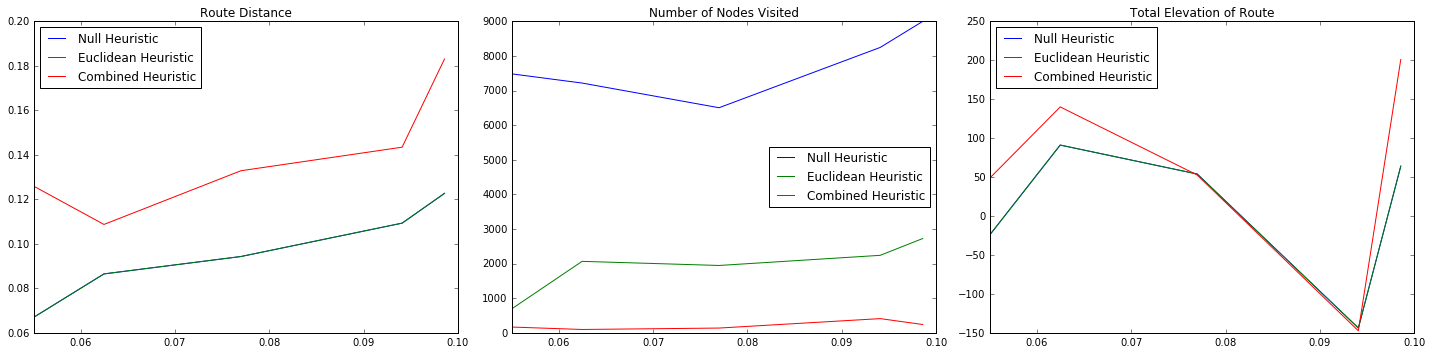
\includegraphics[width=1\textwidth]{../images/cost_1.png}
\end{figure}

\begin{figure}[H]
\caption{Safety road cost under three different heuristics. Again, we expect to see the combined heuristic underperform the null heuristic and euclidean heuristic as the heuristic does not properly model the cost function and is neither admissible nor consistent }
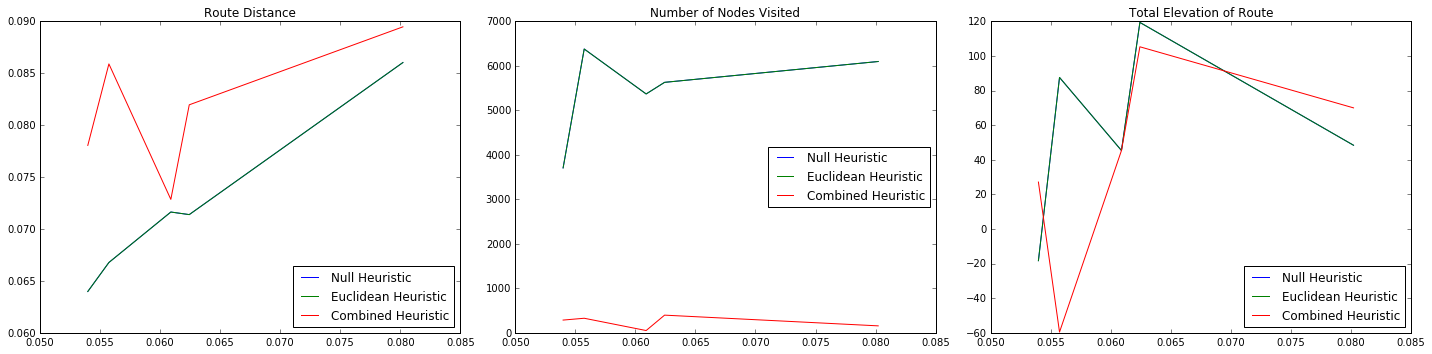
\includegraphics[width=1\textwidth]{../images/cost_2.png}
\end{figure}

\begin{figure}[H]
\caption{Safety, distance, and elevation cost under three different heuristics. Here we still do not expect the combined heuristic to find the ideal solution, as the heuristic is not consistent, but it should do a reasonable job and significantly decrease the nodes expanded.}
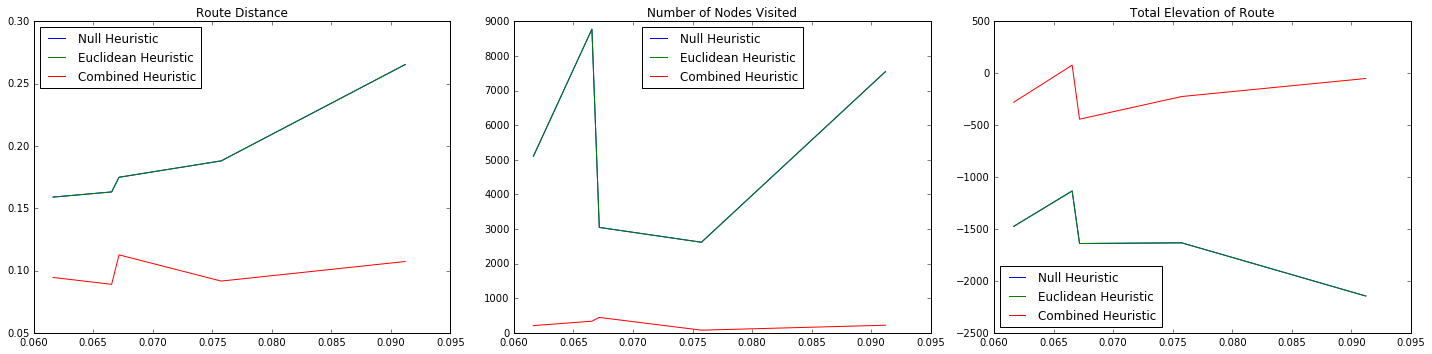
\includegraphics[width=1\textwidth]{../images/cost_3.png}
\end{figure}

\begin{figure}[H]
\caption{Total distance, total nodes expanded, and total elevation change for the three cost functions under uniform cost search.}
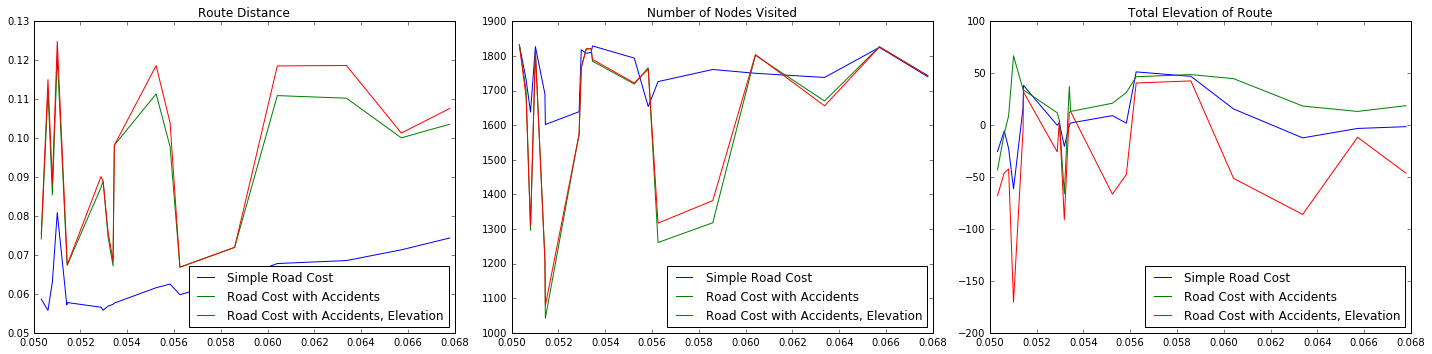
\includegraphics[width=1\textwidth]{../images/total_costs.png}
\end{figure}

TODO: Comparison of K-beam search and Simulated annealing: time to find solution vs total cost of solution found for a number of trials

\section{Discussion}

The graph search approach is a very straightforward and satisfactory solution to this problem. We felt that our results were very reasonable given our preexisting knowledge of Cambridge and San Francisco streets. \\
A couple takeaways from this project:
\begin{itemize}
\item As always, you're only as good as your data. We had some lofty goals for the data that we'd be able to collect and use for this project, but even the data we ended up using was harder to collect and map that we anticipated, and much of the crash data was a few years old. Cambridge and San Francisco are relatively tech-forward cities, so I can imagine this would be even more difficult in most other environments
\item It was interesting to see how our algorithm scaled to the larger map of San Francisco. To plan routes through a larger area, it's clear that we would have to adapt the algorithm to get the runtime within a reasonable range. In particular, we found in our reading that many routing engines actually use inadmissible heuristics for these tasks and still find reasonable results but in a much quicker time.
\end{itemize}

In future work, we could develop faster algorithms by using pruning procedures or finding ways to run expensive operations in parallel or vectorized forms. We could develop more sophisticated models of biking comfort by also including road construction data and pothole reports.

\appendix

\section{System Description}

The easiest way to use our system is to open the provided iPython notebook and run each of the cells. All of the supporting functions can be found in \texttt{final\_project.py}.

\section{Group Makeup}

\begin{enumerate}
\item Nick Hoernle
\begin{enumerate}
\item Creation of graph dictionary structure and A*search algorithm
\item Simulated annealing
\end{enumerate}
\item Nikhila Ravi
\begin{enumerate}
\item K-Beam Search
\item Visualization and analysis of results of graph search algorithms
\end{enumerate}
\item Anna Sophie Hilgard
\begin{enumerate}
\item Construction of Datasets
\item Research and Implementation of more complicated cost functions and heuristics
\end{enumerate}
\end{enumerate}


\bibliographystyle{plain} 
\bibliography{project-template}

\end{document}
